\section*{Appendices}
\begin{frame}{Appendices: Watermarks}
\begin{columns}[c]
\begin{column}{0.48\textwidth}
\textbf{Characteristics:}
    \vfill
    \begin{itemize}
        \item Non-detractive from the original work aesthetics
        \item Inseparable from the original work
    \end{itemize}
\textbf{Purposes of watermark embedding:}
    \vfill
    \begin{itemize}
        \item Marking the manufacturing progress
        \item Protecting the content integrity and authenticity
        \item AI-generation overuse prevention and misinformation protection (recently)
    \end{itemize}
\end{column}

\begin{column}{0.48\textwidth}
\begin{figure}
        \centering      \includegraphics[width=\linewidth]{img/news-watermark.png}
        \caption{New purposes of watermarks}
    \end{figure} 
\end{column}
\end{columns}
\end{frame}

% \begin{frame}{Appendices: Watermarks}
% \begin{columns}[c]
% \begin{column}{0.48\textwidth}
%     \textbf{Characteristics:}
%     \vfill
%     \begin{itemize}
%         \item Non-detractive from the original work aesthetics
%         \item Inseparable from the original work
%     \end{itemize}
%     \vfill
%     \textbf{Purposes of watermark embedding:}
%     \vfill
%     \begin{itemize}
%         \item Marking the manufacturing progress
%         \item Protecting the content integrity and authenticity
%     \end{itemize}
% \end{column}

% \begin{column}{0.48\textwidth}
%     \vfill
%     \begin{figure}
%         \centering
%         \includegraphics[width=\linewidth]{img/papermade-watermark.png}
%         % \caption{Enter Caption}
%     \end{figure}
%     \vfill
% \end{column}

% \end{columns}

% \end{frame}



\begin{frame}{Appendices: Inpainting - GAN-based model}
    \begin{figure}
        \centering
        \includegraphics[width=0.65\linewidth]{img/gan-inpainting.png}
        \caption{GAN-based architecture for image inpainting \footnote{Liu, Hongyu, et al. "Pd-gan: Probabilistic diverse gan for image inpainting." Proceedings of the IEEE/CVF conference on computer vision and pattern recognition. 2021.}}
        \label{fig:enter-label}
    \end{figure}
\end{frame}

\begin{frame}{Appendices: Diffusion-based Models}
    \begin{figure}
        \centering
        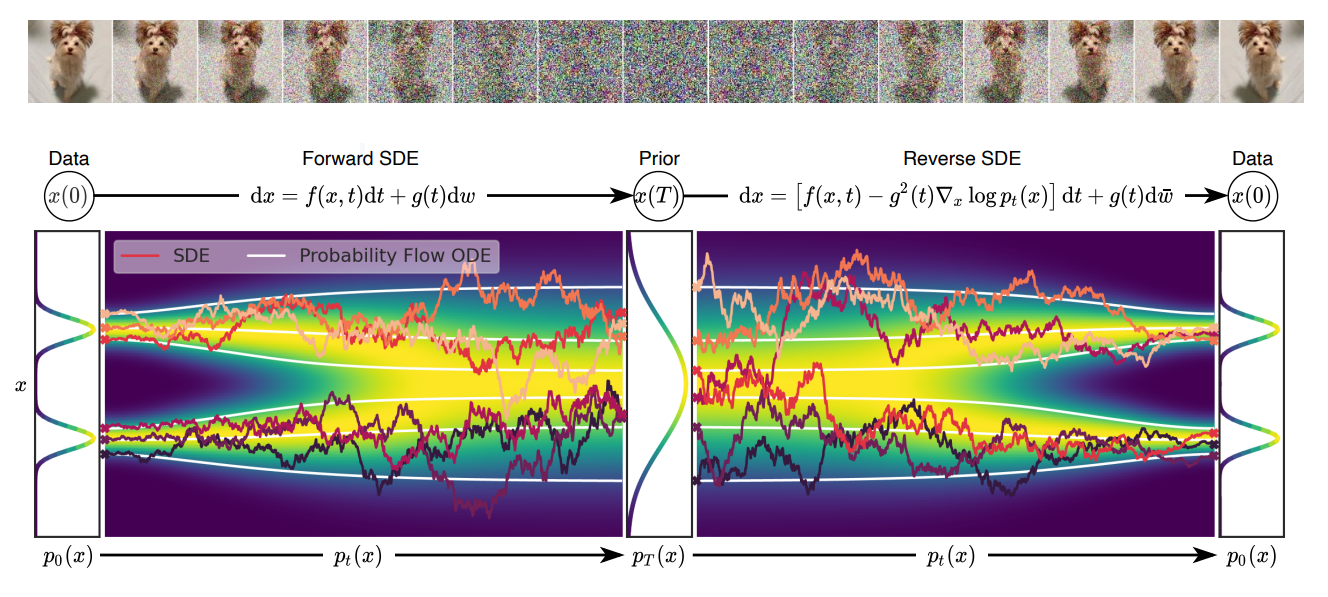
\includegraphics[width=0.85\linewidth]{diffusion.png}
        \caption{Overview of generative modeling through SDEs \footnote{\scriptsize Yang Song and Stefano Ermon. "Generative modeling by estimating gradients of the data distribution." Advances in neural information processing systems 32 (2019).}}  
    \end{figure}
\end{frame}

\begin{frame}{Appendices: Segmentation - U-Net}
    \begin{figure}
        \centering
        \includegraphics[width=0.6\linewidth]{img/unet-segmentation.png}
        \caption{U-Net for image segmentation \footnote{Ronneberger, Olaf, Philipp Fischer, and Thomas Brox. "U-net: Convolutional networks for biomedical image segmentation." Medical image computing and computer-assisted intervention–MICCAI 2015.}}
        \label{fig:enter-label}
    \end{figure}
\end{frame}

\begin{frame}{Appendices: Fully Convolutional Networks (FCN)}
    \begin{figure}
        \centering
        \includegraphics[width=0.75\linewidth]{img/fncc.png}
        \caption{FCN for image segmentation\footnote{Long, Jonathan, Evan Shelhamer, and Trevor Darrell. "Fully convolutional networks for semantic segmentation." Proceedings of the IEEE conference on computer vision and pattern recognition. 2015.}}
        \label{fig:enter-label}
    \end{figure}
\end{frame}

\begin{frame}{Appendices: Segmentation - Vision Transformer (ViT)}
\begin{columns}
    \begin{column}{0.6\textwidth}
        \begin{figure}
            \centering
            \includegraphics[width=\linewidth]{img/vision-transformer.png}
            \caption{Overview of Vision Transformer\footnotemark}
        \end{figure}
    \end{column}
    \begin{column}{0.4\textwidth}
        \begin{align*}
            \text{image}&\xrightarrow{\,\,\,\,\,\,\,\,\,\,\,\,\,\,\,\,\,\,\,\,\,\,\,\,\,\,\,\,\,\,\,\,\,\,\,} \text{patches}\\
                        &\xrightarrow{\text{linear flattening}} \text{sequence of tokens}
        \end{align*}
    \end{column}
\end{columns}
\footnotetext{VDosovitskiy, Alexey, et al. "An image is worth 16x16 words: Transformers for image recognition at scale." arXiv preprint arXiv:2010.11929 (2020).}
\end{frame}

\begin{frame}{Appendices: Stochastic Differential Equations}
    $$\mathrm{d}x(t) = f(x(t),t)\mathrm{d}t + g(x(t),t)\mathrm{d}w,$$
     \begin{columns}[t]
    \begin{column}{0.4\textwidth}
    where,
        \begin{itemize}
            \item $f(x(t),t)$ - the drift coefficient
            \item $g(x(t),t)$ - the diffusion coefficient
            \item $w$ - the Wiener process (Brownian motion)
        \end{itemize}  
    \end{column}
    \begin{column}{0.7\textwidth}
        \begin{figure}
            \centering
            \includegraphics[width=0.7\linewidth]{img/brownian2.png}
            % \caption{Different trajectory of the Brownian motion at the same initial position}
            \label{fig:enter-label}
        \end{figure}
    \end{column}
\end{columns}
\end{frame}

\begin{frame}{Appendices: Forward Process Visualization}
    \begin{figure}
        \centering
        \includegraphics[width=0.8\linewidth]{img/forward_hist2.png}
        \caption{Forward process with histogram visualization}
        \label{fig:enter-label}
    \end{figure}
\end{frame}

\begin{frame}{Appendices: Resource}
\begin{figure}
    \centering
    \includegraphics[width=0.7\linewidth]{img/resources.png}
    \caption{Resources to run diffusion-based models\footnotemark[1]}
    \label{fig:original}
\end{figure}
\footnotetext{\scriptsize Liu, Guan-Horng, et al. "I²SB: Image-to-Image Schrödinger Bridge." arXiv (2023).}
\end{frame}

\begin{frame}{Appendices - Tractability of general SB and SGM}
\begin{figure}
    \centering
    \includegraphics[width=0.6\linewidth]{img/comparision.png}
    \caption{Comparison with others method\footnotemark[1]}
    \label{fig:original}
\end{figure}
\footnotetext{\scriptsize Liu, Guan-Horng, et al. "I²SB: Image-to-Image Schrödinger Bridge." arXiv (2023).}
\end{frame}

\begin{frame}{Appendices: Inpainting Heatmap Visualization}
\setcounter{footnote}{0}
    \begin{figure}
        \centering
        \includegraphics[width = 0.8\textwidth]{img/heatmap_not_in_analys.png}
        \caption{Reconstructed image result through inpainting method with data outside ImageNet dataset \footnotemark}
        \label{fig:enter-label}
    \end{figure}
    \footnotetext{Image from \href{https://www.freepik.com/photos/building}{https://www.freepik.com/photos/building}}
\end{frame}

\begin{frame}{Appendices: Fréchet inception distance (FID)}
The FID between two distributions $p_1$ and $p_2$ is 
$$d^2_F(p_1,p_2)=||\mu_1-\mu_2||^2+\mathrm{tr}(\Sigma_1+\Sigma_2-2(\Sigma_1\Sigma_2)^\frac{1}{2}),$$
where $\mu_i$ and $\Sigma_i$ is the mean and covariance
\end{frame}

\begin{frame}{Appendices: Segmentation Post-processing}
\begin{figure}[t]
    \centering
    \includegraphics[width=\linewidth]{img/dilation-segformer.png}
    %\vspace{0.5cm}
    \caption[SegFormer Segmentation post-processing]{SegFormer Segmentation result with inaccurate mask and post-processing by different dilation kernel}
    \label{fig:segformer-no-dilate}
\end{figure}
\end{frame}

\begin{frame}{Appendices: Segmentation Post-processing}
    \begin{table}[t]
    \centering
    \begin{tabular}{lll}
        \hline
        \multicolumn{1}{c}{\textbf{Method}}                                                & \multicolumn{1}{c}{\textbf{PSNR ↑}} & \multicolumn{1}{c}{\textbf{SSIM ↑}} \\ \hline
        SegFormer + I$^2$SB & 25.13                                & 0.87                                 \\ 
        SegFormer + I$^2$SB + ($3 \times 3$) dilation & {25.81}                       & {0.88}                        \\ 
        SegFormer + I$^2$SB + ($5 \times 5$) dilation & {25.82}                       & {0.88}                        \\ 
        SegFormer + I$^2$SB + ${(7 \times 7)}$ {dilation} & \textbf{27.82}                       & \textbf{0.90}                        \\ 
        SegFormer + I$^2$SB + ($11 \times 11$) dilation & {26.82}                       & {0.89}                        \\ \hline
    \end{tabular}
    \caption{Segmentation post-processing performance with different settings}
    \label{table:segformer-kernel}
\end{table}
\end{frame}

\begin{frame}{Appendices: SWCNN - Watermark Dataset}
    \begin{figure}
        \centering
        \includegraphics[width=0.5\linewidth]{img/Figure2.pdf}
        \caption{Twelve collected watermarks in SWCNN \footnotemark}
    \end{figure}
\footnotetext{Tian, Chunwei, et al. "A self-supervised CNN for image watermark removal." IEEE Transactions on Circuits and Systems for Video Technology (2024).}
\end{frame}

\begin{frame}{Appendices: SWCNN - CNN-based SOTA Watermark Removal}
    \begin{table}[t]
    \centering
    \begin{tabular}{cccll}
        \hline
        \textbf{Methods}                             & \textbf{PSNR ↑}  & \textbf{SSIM ↑} \\ \hline
        FFDNet               & 27.8820          & 0.8778          \\
        DIP                  & 29.7473          & 0.9260          \\
        WGAN-GP               & 31.0752          & 0.9662          \\
        DnCNN               & 30.1071          & 0.9620          \\
        {DRD-Net }                 & 28.9090          & 0.9707          \\
        {FastDerainNet } & 32.2593          & 0.9815          \\
        {EAFNWDD }            & 33.4744          & 0.9700          \\
        \textbf{SWCNN}\footnotemark             & \textbf{36.9022} & \textbf{0.9893} \\ \hline
    \end{tabular}
    \caption[Watermark removal performance of different methods]{Watermark removal performance of different methods compare to SWCNN \footnotemark}
    \label{table:swcnn}
\end{table}
\footnotetext{Tian, Chunwei, et al. "A self-supervised CNN for image watermark removal." IEEE Transactions on Circuits and Systems for Video Technology (2024).}
\end{frame}


\begin{frame}{Appendices: Zero-shot with CLIP}
    \begin{figure}[t]
    \centering
    \includegraphics[width=0.75\linewidth]{img/pic_of_pokemon.png}
    \caption{CLIP\footnotemark attention heatmap with text prompt \textit{The picture have pokemon}}
    \label{fig:pic_of_pokemon}
\end{figure}
\footnotetext{Radford, Alec, et al. "Learning transferable visual models from natural language supervision." International conference on machine learning. PMLR, 2021.}
\end{frame}

\begin{frame}{Appendices: Zero-shot with CLIP}
    \begin{figure}[t]
    \centering
    \includegraphics[width=0.75\linewidth]
    {img/pic_of_wtm.png}
    \caption{CLIP\footnotemark attention heatmap with text prompt \textit{The picture have watermark}}
    \label{fig:pic_of_wtm}
\end{figure}
\footnotetext{Radford, Alec, et al. "Learning transferable visual models from natural language supervision." International conference on machine learning. PMLR, 2021.}
\end{frame}

\begin{frame}{Appendices: Zero-shot Segmentation with Zero-shot Object Detection}
\begin{figure}[t]
    \centering
    \includegraphics[width=0.4\linewidth]{img/groundedsam.png}
    \caption[Zero-shot text prompt result with Object Detection and SAM box prompt]{Zero-shot text prompt \textit{The picture have pokemon} result with Object Detection and SAM box prompt}
    \label{fig:groundedsam}
\end{figure}
\end{frame}

\begin{frame}{Appendices: Zero-shot Segmentation with Finding Visual Task Vectors}
\begin{figure}[t]
    \centering
    \includegraphics[width=0.8\linewidth]{img/FVTV-architecture.png}
    \caption{Zero-shot Segmentation with Finding Visual Task Vectors \footnotemark}
    \label{fig:groundedsam}
\end{figure}
\footnotetext{Hojel, Alberto, et al. "Finding Visual Task Vectors." arXiv preprint arXiv:2404.05729 (2024).}
\end{frame}

\begin{frame}{Appendices: Faster Diffusion Using Wavelet Diffusion}
\begin{figure}[t]
    \centering
    \includegraphics[width=0.5\linewidth]{img/teaser_cifar.png}
    \caption{Comparisons between Wavelet Diffusion method and other GAN and
diffusion techniques in terms of FID and sampling time the on
CIFAR-10 (32 $\times$ 32) dataset.\footnotemark}
    \label{fig:groundedsam}
\end{figure}
\footnotetext{Phung, Hao, Quan Dao, and Anh Tran. "Wavelet diffusion models are fast and scalable image generators." Proceedings of the IEEE/CVF Conference on Computer Vision and Pattern Recognition. 2023.}
\end{frame}

\begin{frame}{Appendices: Faster Diffusion With Diffusion Bridge Implicit Models}
\begin{figure}[t]
    \centering
    \includegraphics[width=0.5\linewidth]{img/DBIM.png}
    \caption{Quantative results in the image restoration task of DBIM and other methods\footnotemark}
    \label{fig:groundedsam}
\end{figure}
\footnotetext{Zheng, Kaiwen, et al. "Diffusion Bridge Implicit Models." arXiv preprint arXiv:2405.15885 (2024).}
\end{frame}

\begin{frame}{Appendices: Structural Similarity Index Measure (SSIM)}
For two image target image $I$ and a noisy predicted image $\hat{I}$, the SSIM index is calculated between two image patches, $x$ and $y$, using the following formula

\begin{equation}
    SSIM(x, y) = [\ell(x, y)]^\alpha \cdot [c(x, y)]^\beta \cdot [s(x, y)]^\gamma,
\end{equation}
where
\begin{itemize}
    \item $\ell(x, y)$ is the luminance comparison function, measuring the closeness of the mean luminance between the two image patches, which has form
          \begin{equation*}
              \ell(x, y) = \frac{2 \mu_x \mu_y + C1}{\mu_x^2 + \mu_y^2 + C1},
          \end{equation*}
          where $\mu_x$ is the average of patch $x$, $\mu_y$ is the average of patch $y$, $C1$ is a small constant (for stability).
\end{itemize}
\end{frame}

\begin{frame}{Appendices: Structural Similarity Index Measure (SSIM)}
For two image target image $I$ and a noisy predicted image $\hat{I}$, the SSIM index is calculated between two image patches, $x$ and $y$, using the following formula

\begin{equation}
    SSIM(x, y) = [\ell(x, y)]^\alpha \cdot [c(x, y)]^\beta \cdot [s(x, y)]^\gamma,
\end{equation}
where
\begin{itemize}
    
    \item  $c(x, y)$ is the contrast comparison function, measuring the similarity of contrast between the patches, which has form
          \begin{equation*}
              c(x, y) = \frac{2 \sigma_x \sigma_y + C2}{\sigma_x^2 + \sigma_y^2 + C2},
          \end{equation*}
          where $\sigma_x$ is the standard deviation of patch $x$, $\sigma_y$ is the standard deviation of patch $y$ and $C2$ is a small constant (for stability)
\end{itemize}
\end{frame}

\begin{frame}{Appendices: Structural Similarity Index Measure (SSIM)}
For two image target image $I$ and a noisy predicted image $\hat{I}$, the SSIM index is calculated between two image patches, $x$ and $y$, using the following formula

\begin{equation}
    SSIM(x, y) = [\ell(x, y)]^\alpha \cdot [c(x, y)]^\beta \cdot [s(x, y)]^\gamma,
\end{equation}
where
\begin{itemize}
    \item $s(x, y)$ is the structure comparison function, measuring the correlation between the patches, which has form
          \begin{equation*}
              s(x, y) = \frac{\sigma_{xy} + C3}{\sigma_x \sigma_y + C3},
          \end{equation*}
          where $\sigma_{xy}$ is the covariance between patches $x$ and $y$ and $C3$ ($C3=\frac{C2}{2}$ in the usual case) is a small constant (for stability)
    \item $\alpha, \beta$, and $\gamma$ are parameters used to control the relative importance of the three components
\end{itemize}
\end{frame}

\begin{frame}{Appendices: Inpainting with I$^2$SB}
\begin{figure}
    \centering
    \includegraphics[width=0.65\linewidth]{img/i2sb-imagenet-result.png}
    \caption{Reconstructed image results through the inpainting method using the I$^{\text{ }2}$SB model with ImageNet dataset}
\end{figure}
\end{frame}

\begin{frame}{Appendices: Morphological Methods}
\begin{figure}[t]
    \centering
    \includegraphics[width=0.55\linewidth]{img/morphologycal.png}
    %\vspace{0.5cm}
    \caption{Morphological methods illustration}
    \label{fig:morphological}
\end{figure}
\end{frame}

\begin{frame}{Appendices: Watermark Embedding Method}
\begin{figure}[t]
    \centering
    \includegraphics[width=0.55\linewidth]{img/wtm_embed_processing.png}
    %\vspace{0.5cm}
    \caption[Watermark image morphological image processing methods]{Watermark image that its object have white detail and its post-processing by using morphological image processing methods}
    \label{fig:wtm-with-white-detail}
\end{figure}
\end{frame}

\begin{frame}{Appendices: Segmentation with Transparent Watermark}
\begin{figure}[t]
    \centering
    \includegraphics[width=0.8\linewidth]{img/transparency_segmentation.png}
    %\vspace{0.5cm}
    \caption{SegFormer Segmentation results with different transparency}
    \label{fig:wtm-with-white-detail}   
\end{figure}
\end{frame}

\begin{frame}{Appendices: Segmentation with Multiple Watermarks}
\begin{figure}[t]
    \centering
    \includegraphics[width=0.5\linewidth]{img/multiple_segmentation.png}
    %\vspace{0.5cm}
    \caption{SegFormer Segmentation results with multiple watermarks in an image}
    \label{fig:wtm-with-white-detail}   
\end{figure}
\end{frame}


\begin{frame}{Appendices: Segmentation with Multiple Transformation of Watermark}
\begin{figure}[t]
    \centering
    \includegraphics[width=0.8\linewidth]{img/segmentation_transformation.jpg}
    %\vspace{0.5cm}
    \caption{SegFormer Segmentation results with multiple transformation of watermark in an image}
    \label{fig:wtm-with-white-detail}   
\end{figure}
\end{frame}

\begin{frame}{Appendices: Inpainting with I$^2$SB}
\begin{figure}
    \centering
    \includegraphics[width=0.8\linewidth]{img/i2sb-imagenet-result.png}
    \caption{Reconstructed image results through the inpainting method using the I$^{\text{ }2}$SB model with \textbf{ImageNet dataset}}
\end{figure}
\end{frame}

\begin{frame}{Appendices: Inpainting with I$^2$SB}
\begin{figure}
    \centering
    \includegraphics[width=0.8\linewidth]{img/i2sb-difference-dataset-result.png}
    \caption{Reconstructed image results through the inpainting method using the I$^{\text{ }2}$SB model with \textbf{unseen} dataset}
\end{figure}
\end{frame}



\begin{frame}{Appendices: Segment Anything}
    \begin{figure}
        \centering
        \includegraphics[width=0.35\linewidth]{img/SAM.png}
        \caption{Segment anything model result with point segmentation\footnote[1]{\scriptsize SAM. Image from https://github.com/facebookresearch/segment-anything}}
        \label{fig:enter-label}
    \end{figure}
\end{frame}
